\documentclass[11pt]{article}
\usepackage[margin=0.72in]{geometry}
\usepackage{booktabs}
\usepackage{longtable}
\usepackage{graphicx}
\usepackage{array}
\usepackage{hyperref}
\usepackage{xcolor}
\hypersetup{colorlinks=true, linkcolor=blue, urlcolor=blue}
\setlength{\parindent}{0pt}
\setlength{\parskip}{6pt}

\title{Archive-2 Raw SPY Options Data EDA}
\author{ML-Based Trading of TP2-Inspired Violations in SPY Call Options}
\date{Generated from professor-provided raw parquet files}

\begin{document}
\maketitle

\section*{Purpose}

This report describes the raw professor-provided Archive-2 dataset before our
project-specific cleaning, TP2 detection, labeling, or ML backtest. The goal is
to understand what data exists, how broad the option chain is, and which raw
data issues must be controlled before using the data for publishable research.

\section*{Raw Source}

\begin{tabular}{ll}
\toprule
Directory & \texttt{Archive-2/spy\_options\_daily/year=*/data.parquet} \\
Dataset in manifest & OPRA.PILLAR \\
Parent symbol & SPY.OPT \\
Date range in files & 2013-04-01 to 2026-06-04 \\
Observed trading sessions & 3,256 \\
Observed raw rows & 58,834,075 \\
Manifest raw rows & 35,758,668 \\
Known vendor gap & 2021-06-18 \\
Skipped-day list size & 56 dates; 1 separate known vendor gap \\
\bottomrule
\end{tabular}

\textbf{Important note.} The manifest reports 35,758,668 rows, while the parquet files currently contain 58,834,075 rows. The report uses the actual parquet
file contents as the source of truth. The difference should be disclosed as a
metadata inconsistency, not as a trading signal.

\section*{What One Raw Row Means}

One raw row is an option quote observation for a SPY option contract on a quote
date. The row contains contract identity, strike, expiration, option type,
bid/ask/mid, quote size, quote timestamp, volume, open interest, SPY close,
dividend metadata, implied volatility, Greeks, forward, and risk-free rate.
The raw files contain multiple rows for many \texttt{quote\_date,
contract\_id} pairs. Therefore, raw row count is not the same thing as
contract-day count. Our final pipeline collapses these raw observations to one
latest-available quote per contract-day before TP2 detection.

\section*{Yearly Coverage and Breadth}

\begin{center}
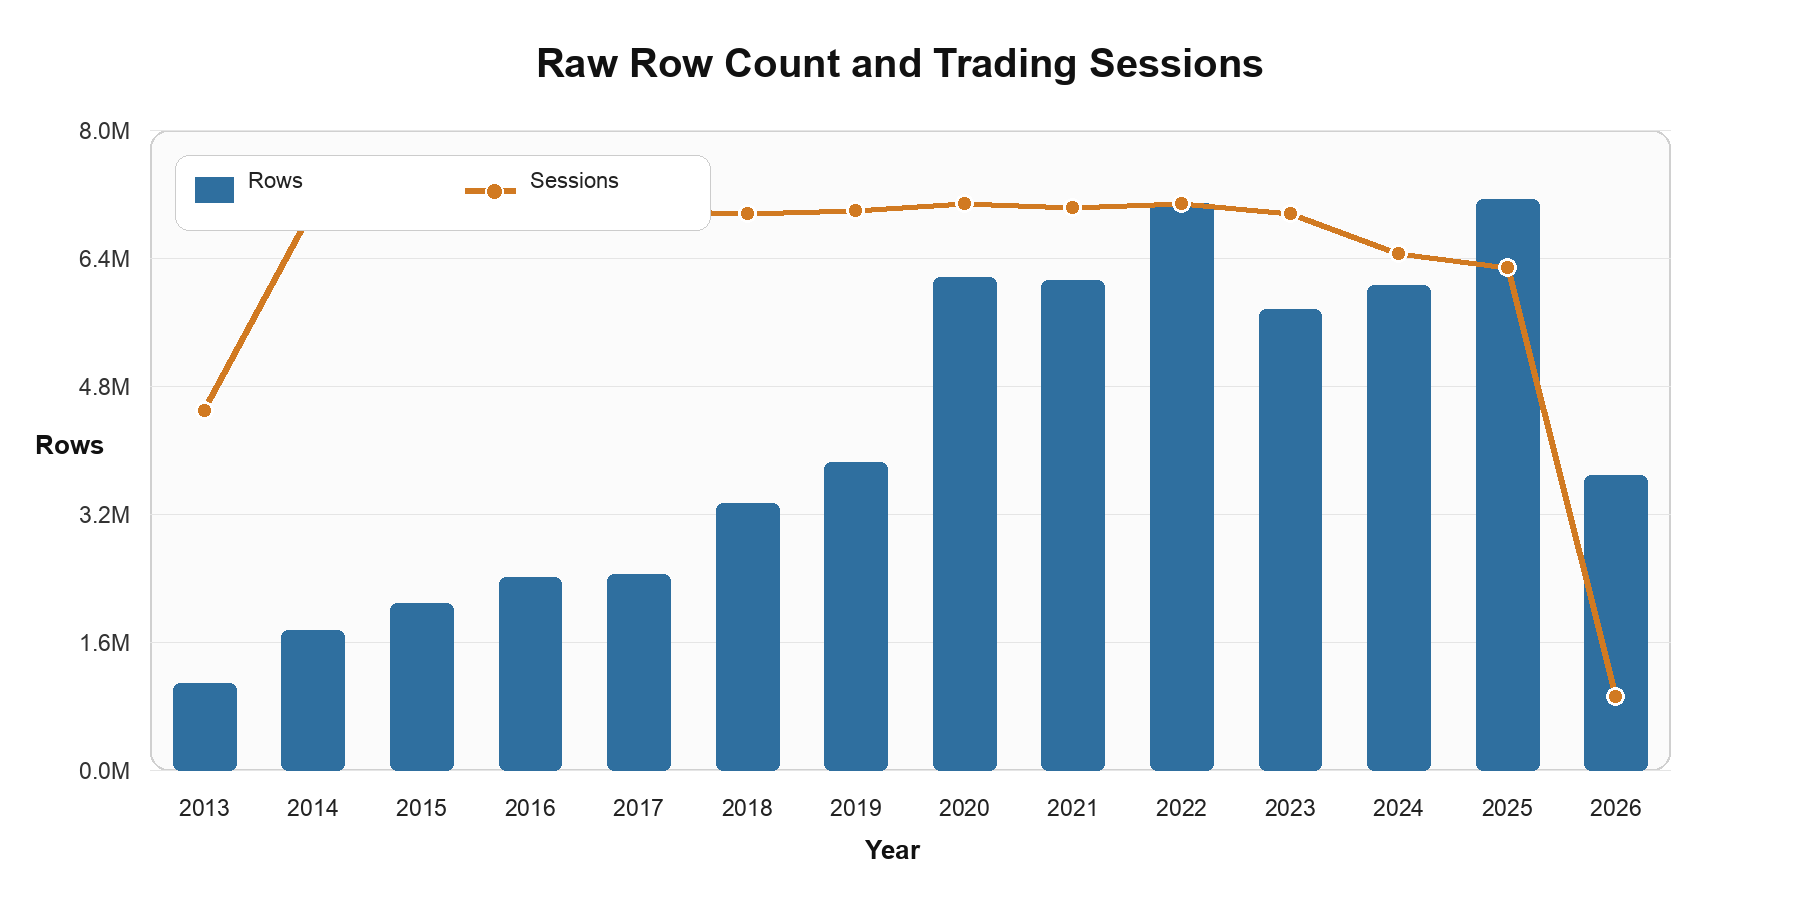
\includegraphics[width=0.98\textwidth]{figures/raw_rows_sessions_by_year.png}
\end{center}

\begin{center}
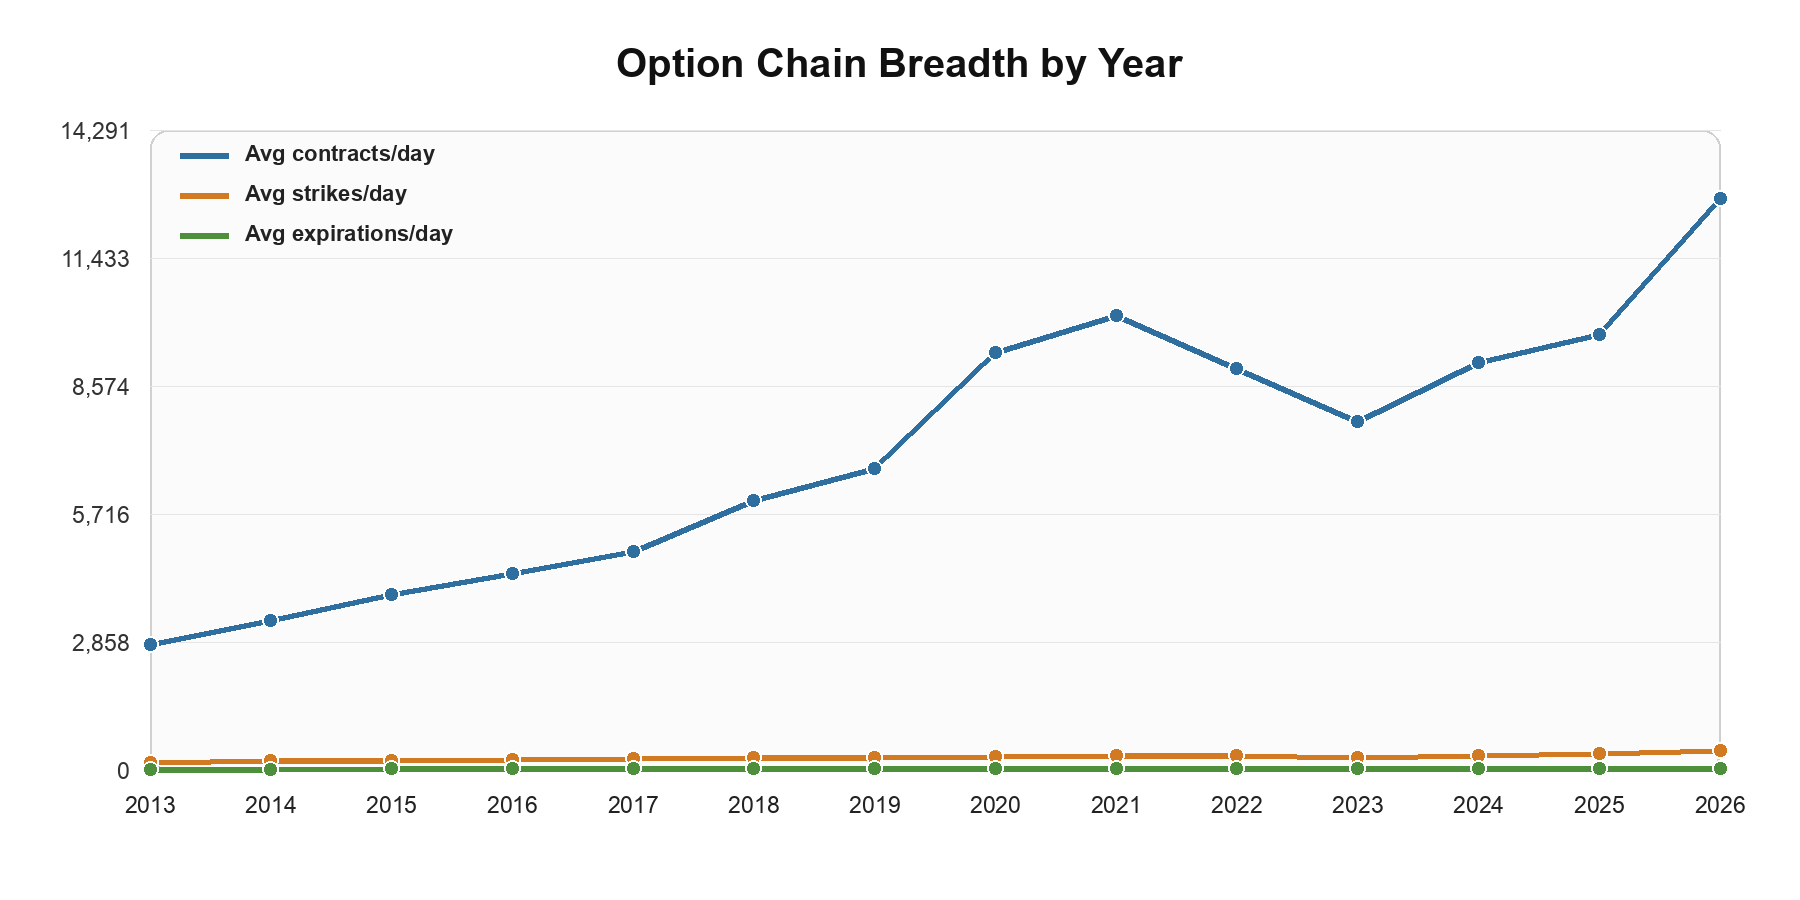
\includegraphics[width=0.98\textwidth]{figures/raw_chain_breadth_by_year.png}
\end{center}

\begingroup
\scriptsize
\begin{longtable}{rrrrrrrrrr}
\toprule
Year & Rows & Sessions & Symbols & Exp. & Strikes & Avg contracts/day & Valid BA & Zero bid & Wide 50 \\
\midrule
2013 & 1,090,018 & 189 & 9,692 & 61 & 227 & 2,803 & 94.8\% & 5.1\% & 8.5\% \\
2014 & 1,741,109 & 249 & 14,494 & 79 & 284 & 3,336 & 95.0\% & 5.0\% & 8.3\% \\
2015 & 2,083,775 & 250 & 17,006 & 79 & 287 & 3,910 & 95.2\% & 4.8\% & 7.9\% \\
2016 & 2,406,752 & 251 & 21,786 & 98 & 314 & 4,379 & 95.4\% & 4.6\% & 7.3\% \\
2017 & 2,441,126 & 249 & 23,974 & 132 & 360 & 4,878 & 95.4\% & 4.6\% & 7.5\% \\
2018 & 3,332,563 & 248 & 37,412 & 181 & 373 & 6,009 & 96.1\% & 3.9\% & 7.1\% \\
2019 & 3,836,239 & 249 & 39,574 & 192 & 395 & 6,722 & 96.8\% & 3.2\% & 5.7\% \\
2020 & 6,143,825 & 251 & 50,864 & 194 & 460 & 9,318 & 98.0\% & 2.0\% & 4.5\% \\
2021 & 6,107,956 & 250 & 53,188 & 190 & 479 & 10,141 & 97.5\% & 2.3\% & 4.5\% \\
2022 & 7,062,256 & 251 & 62,416 & 198 & 392 & 8,974 & 97.4\% & 2.6\% & 5.1\% \\
2023 & 5,746,810 & 248 & 77,952 & 283 & 329 & 7,777 & 92.8\% & 7.2\% & 11.6\% \\
2024 & 6,044,559 & 236 & 76,060 & 286 & 495 & 9,102 & 95.2\% & 4.7\% & 7.4\% \\
2025 & 7,119,099 & 232 & 87,413 & 283 & 649 & 9,728 & 94.9\% & 0.6\% & 3.0\% \\
2026 & 3,677,988 & 103 & 52,383 & 142 & 504 & 12,760 & 93.9\% & 0.0\% & 2.4\% \\
\bottomrule
\end{longtable}
\endgroup

\section*{Quote Quality}

\begin{center}
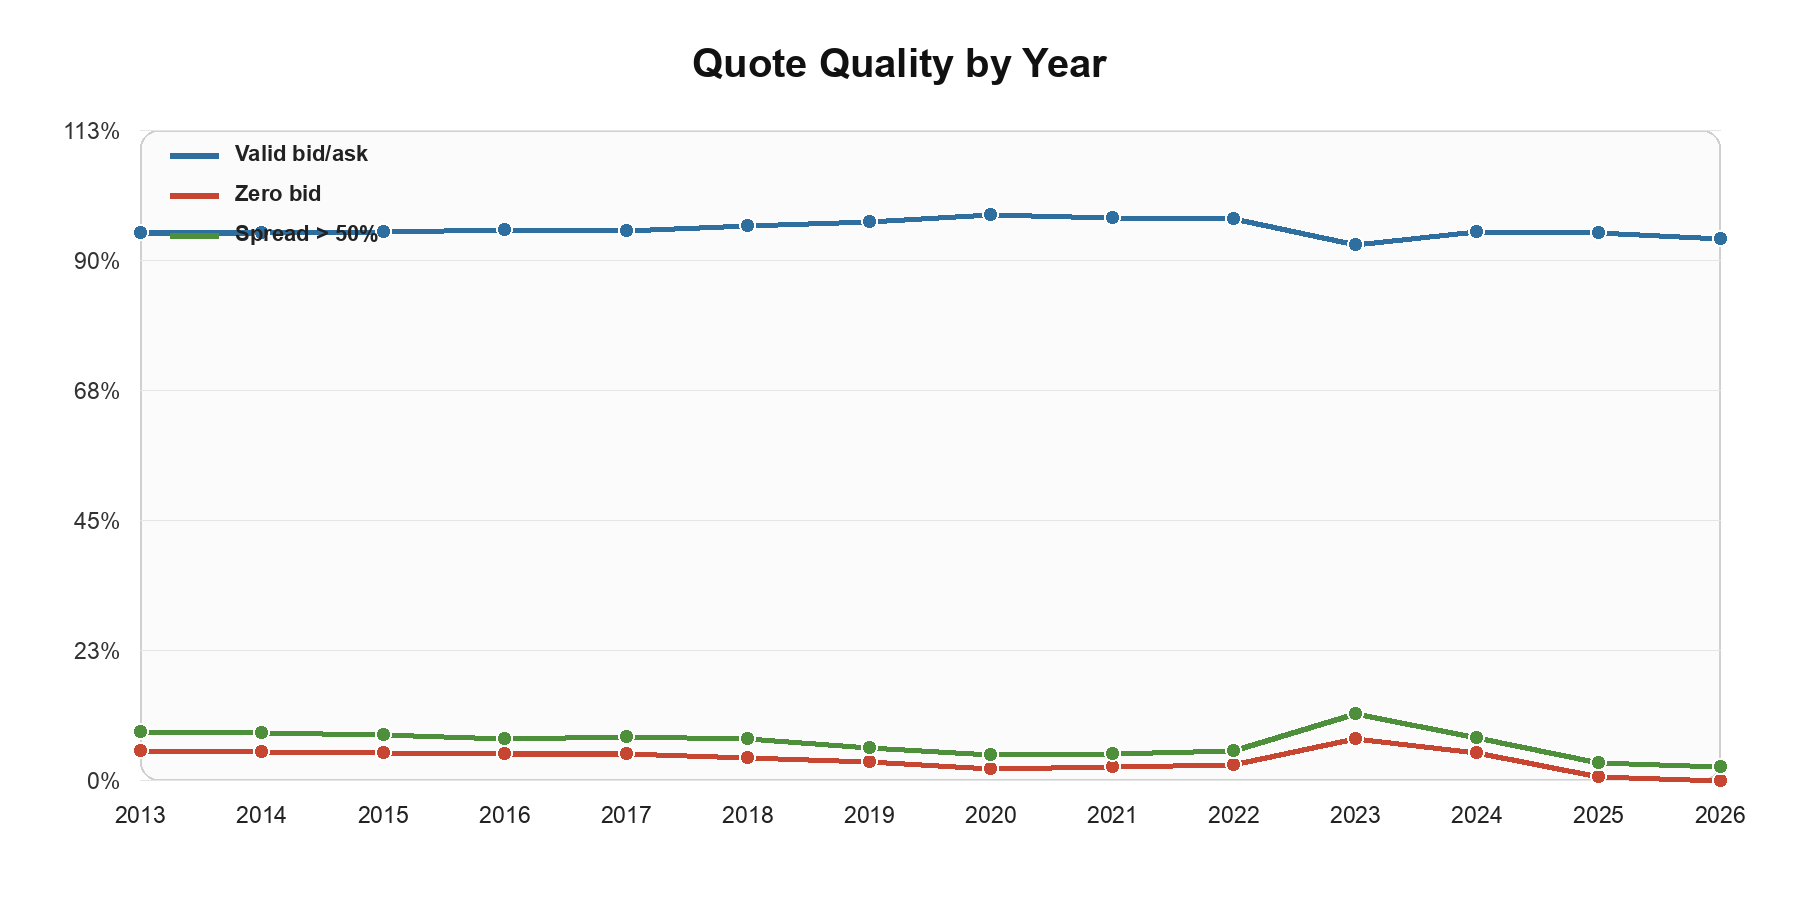
\includegraphics[width=0.98\textwidth]{figures/raw_quote_quality_by_year.png}
\end{center}

Basic bid/ask validity is high in most years, generally above 94\%, but it
drops in 2023 and remains lower in 2026. Wide spreads and zero bids are
material for option data and must be filtered before constructing arbitrage
signals. Crossed quotes are rare, but they exist and should be excluded.

\begingroup
\scriptsize
\begin{longtable}{rrrrr}
\toprule
Year & Duplicate contract-date pairs & Extra raw rows & Extra raw rows pct & Max rows / contract-day \\
\midrule
2013 & 112,365 & 560,299 & 51.4\% & 12 \\
2014 & 179,410 & 910,555 & 52.3\% & 12 \\
2015 & 210,463 & 1,106,161 & 53.1\% & 13 \\
2016 & 249,338 & 1,307,740 & 54.3\% & 14 \\
2017 & 239,234 & 1,226,446 & 50.2\% & 15 \\
2018 & 331,875 & 1,842,311 & 55.3\% & 15 \\
2019 & 386,557 & 2,162,567 & 56.4\% & 16 \\
2020 & 657,136 & 3,805,117 & 61.9\% & 16 \\
2021 & 616,619 & 3,572,644 & 58.5\% & 16 \\
2022 & 696,142 & 4,809,696 & 68.1\% & 16 \\
2023 & 547,666 & 3,818,124 & 66.4\% & 17 \\
2024 & 584,268 & 3,896,583 & 64.5\% & 18 \\
2025 & 678,685 & 4,862,227 & 68.3\% & 18 \\
2026 & 332,240 & 2,363,755 & 64.3\% & 18 \\
\bottomrule
\end{longtable}
\endgroup

The duplicate table should be read as \textbf{multiple raw observations per
contract-day}, not automatically as bad data. It explains why an ingestion
step is necessary: TP2 detection needs one consistent quote per contract-day.

\section*{Detailed Duplicate Diagnostics}

Across the raw parquet files, duplicate contract-day observations appear on
2,566 quote dates. The
total number of extra duplicate rows is 36,244,225.
These are not deleted from the professor data; our ingestion writes a separate
clean research table that collapses each \texttt{quote\_date, contract\_id}
to one final contract-day quote.

\begingroup
\scriptsize
\begin{longtable}{rrrrr}
\toprule
Date & Raw rows & Duplicate pairs & Extra duplicate rows & Max rows same contract-day \\
\midrule
2025-04-08 & 76,747 & 6,986 & 64,612 & 18 \\
2025-04-03 & 67,253 & 6,154 & 56,802 & 18 \\
2025-04-09 & 66,929 & 6,265 & 55,127 & 18 \\
2025-04-07 & 64,151 & 5,988 & 53,439 & 18 \\
2025-04-02 & 57,615 & 5,478 & 47,323 & 18 \\
2026-03-26 & 57,679 & 5,533 & 44,294 & 18 \\
2026-03-19 & 54,848 & 5,190 & 41,968 & 18 \\
2026-03-02 & 54,375 & 5,064 & 41,469 & 18 \\
2026-04-07 & 54,684 & 5,198 & 41,333 & 18 \\
2020-03-17 & 52,752 & 6,232 & 41,312 & 16 \\
2025-11-19 & 51,434 & 4,772 & 40,865 & 18 \\
2020-03-11 & 51,369 & 6,009 & 40,771 & 16 \\
2025-04-15 & 52,198 & 5,093 & 40,209 & 18 \\
2025-03-10 & 50,467 & 5,063 & 40,198 & 18 \\
2026-04-16 & 53,217 & 5,451 & 39,942 & 18 \\
\bottomrule
\end{longtable}
\endgroup

\begingroup
\scriptsize
\begin{longtable}{rrrrr}
\toprule
Year & Date & Contract ID & Option symbol & Raw rows same contract-day \\
\midrule
2024 & 2024-08-21 & 1392510222 & SPY   250815P00630000 & 18 \\
2024 & 2024-09-12 & 1308623527 & SPY   240930C00504000 & 18 \\
2024 & 2024-09-12 & 1308623695 & SPY   240930C00501000 & 18 \\
2024 & 2024-09-12 & 1375731761 & SPY   240930P00407000 & 18 \\
2024 & 2024-09-12 & 1375732694 & SPY   240930P00406000 & 18 \\
2024 & 2024-09-12 & 1375731937 & SPY   240930P00380000 & 18 \\
2024 & 2024-09-12 & 1375731980 & SPY   240930P00395000 & 18 \\
2024 & 2024-09-12 & 1308623095 & SPY   240930C00394000 & 18 \\
2024 & 2024-09-12 & 1308622867 & SPY   240930C00510000 & 18 \\
2024 & 2024-10-08 & 1342178697 & SPY   241016C00484000 & 18 \\
2024 & 2024-10-08 & 1409286620 & SPY   241014P00590000 & 18 \\
2024 & 2024-10-08 & 1392510295 & SPY   241015P00420000 & 18 \\
2024 & 2024-10-08 & 1325401530 & SPY   241015C00483000 & 18 \\
2024 & 2024-10-08 & 1342178390 & SPY   241016C00465000 & 18 \\
2024 & 2024-10-08 & 1342178434 & SPY   241016C00496000 & 18 \\
2024 & 2024-10-08 & 1409286229 & SPY   241016P00630000 & 18 \\
2024 & 2024-10-08 & 1325401273 & SPY   241017C00310000 & 18 \\
2024 & 2024-10-08 & 1409286534 & SPY   241018P00416000 & 18 \\
2024 & 2024-10-08 & 1342177569 & SPY   241018C00434000 & 18 \\
2024 & 2024-10-08 & 1342178418 & SPY   241014C00494000 & 18 \\
\bottomrule
\end{longtable}
\endgroup

\section*{Quote Time Distribution}

\begingroup
\scriptsize
\begin{longtable}{rrrrrr}
\toprule
Year & 09:30--10:00 & 10:00--12:00 & 12:00--15:00 & 15:00--15:55 & 15:55--16:00 \\
\midrule
2013 & 1.3\% & 4.6\% & 11.9\% & 21.3\% & 27.5\% \\
2014 & 1.4\% & 4.7\% & 12.6\% & 23.8\% & 24.7\% \\
2015 & 1.3\% & 4.3\% & 11.8\% & 23.7\% & 26.9\% \\
2016 & 1.2\% & 4.5\% & 12.3\% & 24.9\% & 27.0\% \\
2017 & 1.3\% & 4.9\% & 12.4\% & 23.4\% & 23.1\% \\
2018 & 1.3\% & 4.4\% & 12.3\% & 25.7\% & 26.9\% \\
2019 & 1.3\% & 4.7\% & 12.7\% & 24.2\% & 28.4\% \\
2020 & 1.3\% & 4.2\% & 12.0\% & 25.6\% & 34.7\% \\
2021 & 1.4\% & 4.5\% & 12.7\% & 24.4\% & 30.9\% \\
2022 & 1.1\% & 3.6\% & 11.3\% & 27.5\% & 38.6\% \\
2023 & 1.9\% & 5.1\% & 11.7\% & 18.9\% & 21.6\% \\
2024 & 2.5\% & 6.3\% & 12.8\% & 15.7\% & 12.5\% \\
2025 & 2.4\% & 6.3\% & 13.5\% & 17.1\% & 13.8\% \\
2026 & 2.1\% & 5.8\% & 11.8\% & 15.3\% & 11.4\% \\
\bottomrule
\end{longtable}
\endgroup

The raw archive is not a single clean close snapshot. Many rows have quote
times before the final five minutes, and some rows have missing quote-time
bucket values. After reviewing this behavior, the active clean dataset now uses
the latest available quote per contract-day rather than a hard 15:55 cutoff.

\section*{Missing or Skipped Sessions}

The raw archive metadata lists 57 skipped or missing
session dates. Some are normal early-close dates, and one is explicitly listed
as a known vendor gap. A direct raw-date presence check found 0
of these dates present and 57 absent in the raw daily summary,
with no 15:55 filter applied. The project does not fabricate missing sessions.

\begingroup
\scriptsize
\begin{longtable}{rll}
\toprule
Date & Known vendor gap & Note \\
\midrule
2013-07-03 & 0 & Listed by raw archive metadata as skipped/not present \\
2013-11-29 & 0 & Listed by raw archive metadata as skipped/not present \\
2013-12-24 & 0 & Listed by raw archive metadata as skipped/not present \\
2014-07-03 & 0 & Listed by raw archive metadata as skipped/not present \\
2014-11-28 & 0 & Listed by raw archive metadata as skipped/not present \\
2014-12-24 & 0 & Listed by raw archive metadata as skipped/not present \\
2015-11-27 & 0 & Listed by raw archive metadata as skipped/not present \\
2015-12-24 & 0 & Listed by raw archive metadata as skipped/not present \\
2016-11-25 & 0 & Listed by raw archive metadata as skipped/not present \\
2017-07-03 & 0 & Listed by raw archive metadata as skipped/not present \\
2017-11-24 & 0 & Listed by raw archive metadata as skipped/not present \\
2018-07-03 & 0 & Listed by raw archive metadata as skipped/not present \\
2018-11-23 & 0 & Listed by raw archive metadata as skipped/not present \\
2018-12-24 & 0 & Listed by raw archive metadata as skipped/not present \\
2019-07-03 & 0 & Listed by raw archive metadata as skipped/not present \\
2019-11-29 & 0 & Listed by raw archive metadata as skipped/not present \\
2019-12-24 & 0 & Listed by raw archive metadata as skipped/not present \\
2020-11-27 & 0 & Listed by raw archive metadata as skipped/not present \\
2020-12-24 & 0 & Listed by raw archive metadata as skipped/not present \\
2021-06-18 & 1 & Known vendor gap listed by raw archive metadata \\
2021-11-26 & 0 & Listed by raw archive metadata as skipped/not present \\
2023-07-03 & 0 & Listed by raw archive metadata as skipped/not present \\
2023-11-24 & 0 & Listed by raw archive metadata as skipped/not present \\
2024-04-04 & 0 & Listed by raw archive metadata as skipped/not present \\
2024-04-11 & 0 & Listed by raw archive metadata as skipped/not present \\
2024-06-11 & 0 & Listed by raw archive metadata as skipped/not present \\
2024-06-14 & 0 & Listed by raw archive metadata as skipped/not present \\
2024-06-17 & 0 & Listed by raw archive metadata as skipped/not present \\
2024-06-20 & 0 & Listed by raw archive metadata as skipped/not present \\
2024-06-26 & 0 & Listed by raw archive metadata as skipped/not present \\
2024-06-27 & 0 & Listed by raw archive metadata as skipped/not present \\
2024-06-28 & 0 & Listed by raw archive metadata as skipped/not present \\
2024-07-02 & 0 & Listed by raw archive metadata as skipped/not present \\
2024-07-03 & 0 & Listed by raw archive metadata as skipped/not present \\
2024-07-05 & 0 & Listed by raw archive metadata as skipped/not present \\
2024-07-08 & 0 & Listed by raw archive metadata as skipped/not present \\
2024-08-22 & 0 & Listed by raw archive metadata as skipped/not present \\
2024-11-29 & 0 & Listed by raw archive metadata as skipped/not present \\
2024-12-24 & 0 & Listed by raw archive metadata as skipped/not present \\
2025-03-11 & 0 & Listed by raw archive metadata as skipped/not present \\
2025-04-10 & 0 & Listed by raw archive metadata as skipped/not present \\
2025-07-03 & 0 & Listed by raw archive metadata as skipped/not present \\
2025-07-15 & 0 & Listed by raw archive metadata as skipped/not present \\
2025-07-16 & 0 & Listed by raw archive metadata as skipped/not present \\
2025-08-11 & 0 & Listed by raw archive metadata as skipped/not present \\
2025-08-19 & 0 & Listed by raw archive metadata as skipped/not present \\
2025-09-05 & 0 & Listed by raw archive metadata as skipped/not present \\
2025-09-10 & 0 & Listed by raw archive metadata as skipped/not present \\
2025-09-12 & 0 & Listed by raw archive metadata as skipped/not present \\
2025-09-15 & 0 & Listed by raw archive metadata as skipped/not present \\
2025-09-25 & 0 & Listed by raw archive metadata as skipped/not present \\
2025-10-08 & 0 & Listed by raw archive metadata as skipped/not present \\
2025-10-09 & 0 & Listed by raw archive metadata as skipped/not present \\
2025-10-13 & 0 & Listed by raw archive metadata as skipped/not present \\
2025-11-28 & 0 & Listed by raw archive metadata as skipped/not present \\
2025-12-17 & 0 & Listed by raw archive metadata as skipped/not present \\
2025-12-24 & 0 & Listed by raw archive metadata as skipped/not present \\
\bottomrule
\end{longtable}
\endgroup

\section*{Date-Level Quote Problems}

The next tables identify the most affected dates in the raw archive. These are
diagnostic tables for data understanding; the final trading pipeline handles
them through quote cleaning, bid/ask filters, and invalid-exit accounting.

\begingroup
\scriptsize
\begin{longtable}{rrrrr}
\toprule
Date & Raw rows & Invalid bid/ask rows & Invalid bid/ask pct & Zero bid pct \\
\midrule
2021-12-02 & 39,008 & 7,473 & 19.2\% & 1.2\% \\
2016-02-19 & 4,504 & 670 & 14.9\% & 14.9\% \\
2016-02-05 & 4,690 & 666 & 14.2\% & 14.2\% \\
2016-01-29 & 4,858 & 682 & 14.0\% & 14.0\% \\
2016-02-12 & 4,666 & 649 & 13.9\% & 13.9\% \\
2018-03-16 & 6,438 & 887 & 13.8\% & 13.8\% \\
2013-11-08 & 2,914 & 399 & 13.7\% & 13.7\% \\
2014-10-03 & 3,670 & 489 & 13.3\% & 13.3\% \\
2018-05-11 & 6,812 & 905 & 13.3\% & 13.3\% \\
2016-03-18 & 4,172 & 553 & 13.3\% & 13.3\% \\
2014-09-26 & 3,524 & 466 & 13.2\% & 13.2\% \\
2016-02-26 & 4,344 & 574 & 13.2\% & 13.2\% \\
2013-06-21 & 2,744 & 362 & 13.2\% & 13.2\% \\
2016-03-04 & 4,284 & 565 & 13.2\% & 13.2\% \\
2014-10-10 & 3,682 & 483 & 13.1\% & 13.1\% \\
\bottomrule
\end{longtable}
\endgroup

\begingroup
\scriptsize
\begin{longtable}{rrrrr}
\toprule
Date & Raw rows & Wide 50 rows & Wide 50 pct & Crossed rows \\
\midrule
2018-03-16 & 6,438 & 1,401 & 21.8\% & 0 \\
2020-02-28 & 9,242 & 1,878 & 20.3\% & 10 \\
2018-05-11 & 6,812 & 1,373 & 20.2\% & 0 \\
2018-02-05 & 22,758 & 4,446 & 19.5\% & 0 \\
2013-11-08 & 2,914 & 561 & 19.3\% & 1 \\
2020-03-13 & 11,496 & 2,210 & 19.2\% & 0 \\
2020-03-20 & 11,758 & 2,258 & 19.2\% & 0 \\
2018-06-29 & 6,048 & 1,158 & 19.1\% & 0 \\
2016-01-29 & 4,858 & 929 & 19.1\% & 0 \\
2016-02-19 & 4,504 & 836 & 18.6\% & 0 \\
2017-06-02 & 5,070 & 940 & 18.5\% & 0 \\
2018-05-25 & 6,240 & 1,131 & 18.1\% & 0 \\
2014-12-19 & 3,604 & 653 & 18.1\% & 0 \\
2013-09-20 & 3,032 & 548 & 18.1\% & 0 \\
2013-09-27 & 3,126 & 560 & 17.9\% & 0 \\
\bottomrule
\end{longtable}
\endgroup

\section*{Maturity Distribution}

\begin{center}
\begin{tabular}{lrr}
\toprule
DTE bucket & Rows & Percent \\
\midrule
0DTE & 1,556,512 & 2.6\% \\
1-2Y & 4,379,634 & 7.4\% \\
1-7DTE & 6,936,039 & 11.8\% \\
181-365DTE & 6,748,753 & 11.5\% \\
2Y+ & 1,542,629 & 2.6\% \\
31-60DTE & 8,192,949 & 13.9\% \\
61-90DTE & 4,092,316 & 7.0\% \\
8-30DTE & 16,993,718 & 28.9\% \\
91-180DTE & 7,461,334 & 12.7\% \\
expired/negative & 930,191 & 1.6\% \\
\bottomrule
\end{tabular}
\end{center}

The archive covers short-dated and long-dated SPY options. Our TP2 research
pipeline restricts the usable universe to a controlled DTE range so that
illiquid long tails and near-expiration edge cases do not dominate the signal.

\section*{Missingness in Model-Relevant Columns}

\begingroup
\scriptsize
\begin{longtable}{rrrrrrr}
\toprule
Year & IV miss & Delta miss & Theta miss & Vega miss & OI miss & Rate miss \\
\midrule
2013 & 10.9\% & 10.9\% & 10.9\% & 10.9\% & 0.0\% & 0.1\% \\
2014 & 10.5\% & 10.5\% & 10.5\% & 10.5\% & 0.0\% & 0.1\% \\
2015 & 8.2\% & 8.2\% & 8.2\% & 8.2\% & 0.0\% & 0.2\% \\
2016 & 7.8\% & 7.8\% & 7.8\% & 7.8\% & 0.0\% & 0.2\% \\
2017 & 9.9\% & 9.9\% & 9.9\% & 9.9\% & 0.0\% & 0.3\% \\
2018 & 5.0\% & 5.0\% & 5.0\% & 5.0\% & 0.0\% & 0.5\% \\
2019 & 4.3\% & 4.3\% & 4.3\% & 4.3\% & 0.0\% & 0.4\% \\
2020 & 4.8\% & 4.8\% & 4.8\% & 4.8\% & 0.0\% & 0.3\% \\
2021 & 7.5\% & 7.5\% & 7.5\% & 7.5\% & 0.0\% & 0.3\% \\
2022 & 3.5\% & 3.5\% & 3.5\% & 3.5\% & 0.0\% & 0.4\% \\
2023 & 6.3\% & 6.3\% & 6.3\% & 6.3\% & 0.0\% & 1.1\% \\
2024 & 7.7\% & 7.7\% & 7.7\% & 7.7\% & 2.4\% & 1.4\% \\
2025 & 11.5\% & 11.5\% & 11.5\% & 11.5\% & 2.7\% & 1.3\% \\
2026 & 14.9\% & 14.9\% & 14.9\% & 14.9\% & 2.2\% & 1.2\% \\
\bottomrule
\end{longtable}
\endgroup

Greeks and implied volatility are useful model features, but they are not
always available. They should be treated as optional/derived features with
missingness controls, not as mandatory raw fields for defining option prices or
TP2 violations.

\section*{Date-Level Missingness}

At least one key field is missing on 3,256
raw sessions. This is mostly because implied volatility, Greeks, risk-free
rate, and open interest are not complete for every contract. Bid, ask, mid,
volume, and SPY close are much more complete and are the required fields for
pricing and TP2 construction.

\begingroup
\scriptsize
\begin{longtable}{rlrrr}
\toprule
Date & Column & Raw rows & Missing rows & Missing pct \\
\midrule
2026-03-26 & next\_div\_amount & 57,679 & 57,679 & 100.0\% \\
2026-03-26 & next\_ex\_div\_date & 57,679 & 57,679 & 100.0\% \\
2026-04-07 & next\_div\_amount & 54,684 & 54,684 & 100.0\% \\
2026-04-07 & next\_ex\_div\_date & 54,684 & 54,684 & 100.0\% \\
2026-04-16 & next\_div\_amount & 53,217 & 53,217 & 100.0\% \\
2026-04-16 & next\_ex\_div\_date & 53,217 & 53,217 & 100.0\% \\
2026-03-30 & next\_div\_amount & 51,639 & 51,639 & 100.0\% \\
2026-03-30 & next\_ex\_div\_date & 51,639 & 51,639 & 100.0\% \\
2026-04-14 & next\_div\_amount & 48,761 & 48,761 & 100.0\% \\
2026-04-14 & next\_ex\_div\_date & 48,761 & 48,761 & 100.0\% \\
2026-03-25 & next\_div\_amount & 48,280 & 48,280 & 100.0\% \\
2026-03-25 & next\_ex\_div\_date & 48,280 & 48,280 & 100.0\% \\
2026-03-31 & next\_div\_amount & 47,370 & 47,370 & 100.0\% \\
2026-03-31 & next\_ex\_div\_date & 47,370 & 47,370 & 100.0\% \\
2026-05-05 & next\_div\_amount & 46,783 & 46,783 & 100.0\% \\
2026-05-05 & next\_ex\_div\_date & 46,783 & 46,783 & 100.0\% \\
2026-05-14 & next\_div\_amount & 46,219 & 46,219 & 100.0\% \\
2026-05-14 & next\_ex\_div\_date & 46,219 & 46,219 & 100.0\% \\
2026-04-08 & next\_div\_amount & 46,181 & 46,181 & 100.0\% \\
2026-04-08 & next\_ex\_div\_date & 46,181 & 46,181 & 100.0\% \\
\bottomrule
\end{longtable}
\endgroup

\section*{Clean Dataset Version for Next Pipeline}

After reviewing the raw quote-time distribution, the next pipeline version
should use the latest available raw quote for each contract-day rather than
requiring the quote time to be at or after 15:55. The data provider appears to
store the latest scraped quote available for that contract-day, even when the
timestamp is earlier than 15:55. Therefore the new clean dataset keeps the
last available quote after duplicate collapse, while preserving the same
research filters: SPY calls only, DTE 1--90, valid bid/ask, positive bid, and
spread percentage no greater than 50\%.

\begingroup
\scriptsize
\begin{longtable}{lrrrrrr}
\toprule
Dataset version & Rows & Sessions & Duplicate rows & Call rows & Min DTE & Max DTE \\
\midrule
Old near-close >=15:55 & 804,809 & 3,255 & 0 & 804,809 & 1 & 90 \\
New last-available quote & 4,912,891 & 3,256 & 0 & 4,912,891 & 1 & 90 \\
\bottomrule
\end{longtable}
\endgroup

The active reconstructed file for the next structural pipeline work is:
\begin{quote}
\small\path{data/processed/archive2_spy_call_allmoneyness_lastquote_clean_2013_2026.parquet}
\end{quote}

\section*{TP2 Inequality Audit Before Violation Charts}

Before adding violation counts by year or month, we verified the call-side TP2
condition against the Glasserman--Li--Pirjol formulation. For calls with
$T_1<T_2$ and $K_1/F_{T_1}<K_2/F_{T_2}$, the no-violation condition is

\[
C(K_1,T_1)C(K_2,T_2)
\geq
C(K_1F_{T_2}/F_{T_1},T_2)C(K_2F_{T_1}/F_{T_2},T_1).
\]

Therefore, the call violation condition is

\[
\mathrm{LHS} < \mathrm{RHS}.
\]

The current forward-adjusted detector implements exactly this direction:
\texttt{lhs = A\_mid * B\_mid},
\texttt{rhs = C\_mid * D\_mid}, and keeps call rows with
\texttt{lhs < rhs} and positive normalized severity. The January 2--5, 2024
smoke test on the last-available clean dataset produced 661 violation rows;
all 661 satisfied \texttt{lhs < rhs}, all satisfied
$K_1/F_{T_1}<K_2/F_{T_2}$, and all had $T_1<T_2$. This means yearly and monthly
violation charts can be added after running the full detector on the new active
dataset.

\section*{TP2 Violation Counts on Active Last-Available Dataset}

The full forward-adjusted TP2 detector was run on the active clean dataset:
\begin{quote}
\small\path{data/processed/archive2_spy_call_allmoneyness_lastquote_clean_2013_2026.parquet}
\end{quote}

Detector settings were all SPY calls, DTE 1--90, positive bid, valid bid/ask,
spread percentage no greater than 50\%, latest available quote per
contract-day, maximum 80 strikes per expiration, and minimum normalized
severity of 0.0001. The detector output contains 2,430,220 daily TP2 violation
feature rows across 2013--2026. A validation pass over the 14 yearly parquet
outputs found zero rows with \texttt{lhs >= rhs}, zero rows with invalid
expiration ordering, and zero duplicate \texttt{violation\_id} values.

\textbf{Interpretation.} These are daily rectangle-level violation rows, not
unique arbitrage episodes and not executed trades. The same economic rectangle
can appear on multiple adjacent trading days. The next structural pipeline step
should therefore convert daily rows into episode-level observations before ML
labeling and trading backtests.

\begin{center}
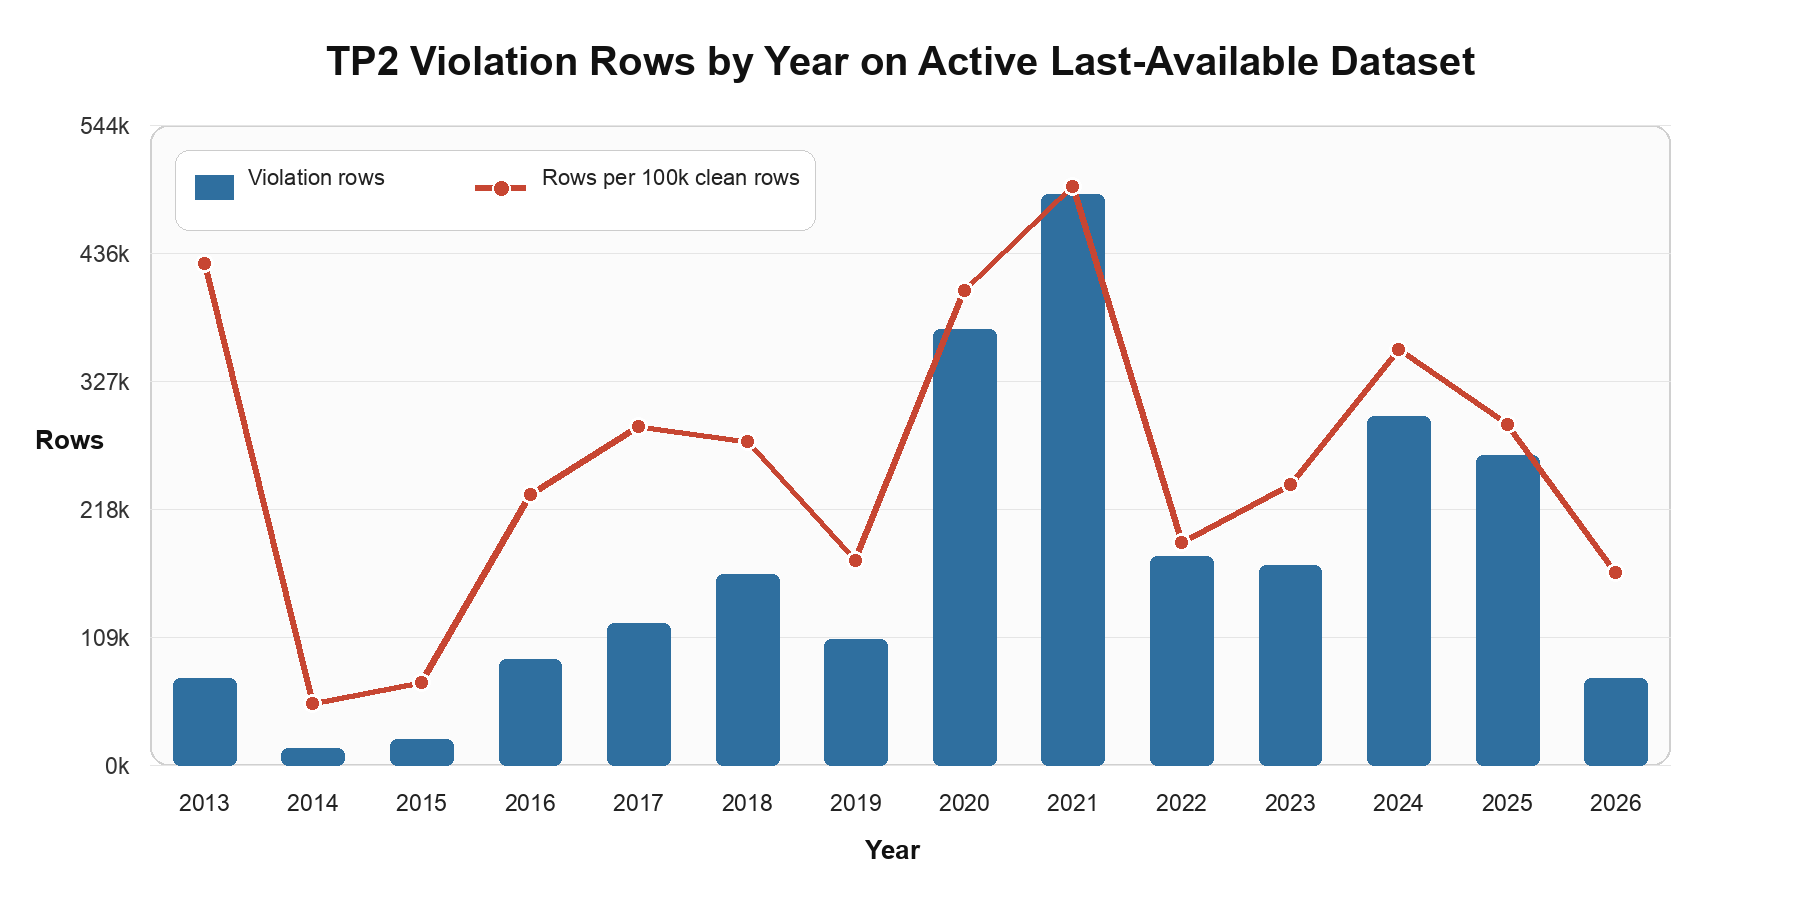
\includegraphics[width=0.98\textwidth]{figures/lastquote_tp2_violations_by_year.png}
\end{center}

\begin{center}
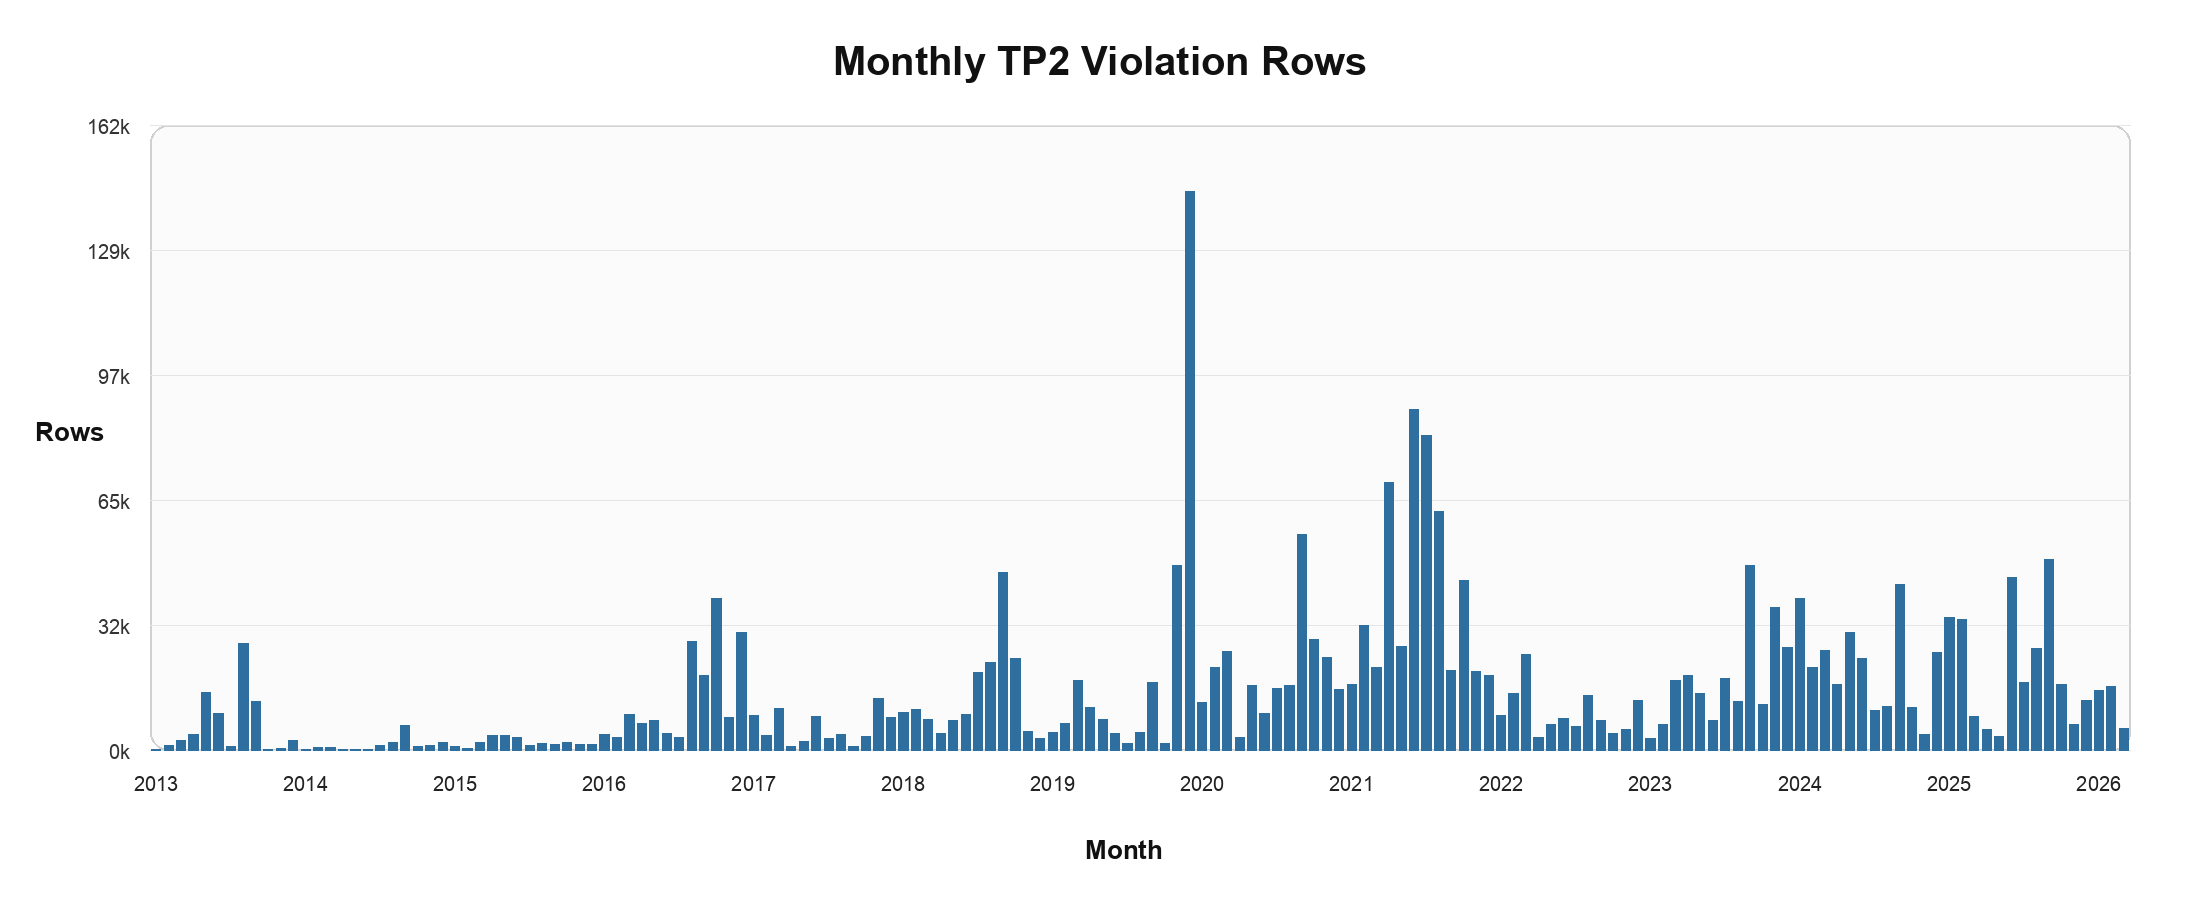
\includegraphics[width=0.98\textwidth]{figures/lastquote_tp2_violations_by_month.png}
\end{center}

\begingroup
\scriptsize
\begin{longtable}{rrrrrrr}
\toprule
Year & Clean rows & Sessions & Violation rows & Violation sessions & Rows/session & Rows/100k clean \\
\midrule
2013 & 99,129 & 189 & 73,619 & 126 & 389.5 & 74,266 \\
2014 & 156,479 & 249 & 14,161 & 158 & 56.9 & 9,050 \\
2015 & 181,555 & 250 & 22,101 & 235 & 88.4 & 12,173 \\
2016 & 225,307 & 251 & 90,011 & 250 & 358.6 & 39,950 \\
2017 & 242,041 & 249 & 121,186 & 246 & 486.7 & 50,068 \\
2018 & 340,904 & 248 & 162,873 & 248 & 656.7 & 47,777 \\
2019 & 355,517 & 249 & 107,568 & 249 & 432.0 & 30,257 \\
2020 & 528,083 & 251 & 370,574 & 250 & 1,476.4 & 70,173 \\
2021 & 567,934 & 250 & 486,076 & 250 & 1,944.3 & 85,587 \\
2022 & 539,482 & 251 & 177,497 & 251 & 707.2 & 32,901 \\
2023 & 410,310 & 248 & 169,882 & 248 & 685.0 & 41,403 \\
2024 & 483,658 & 236 & 297,226 & 236 & 1,259.4 & 61,454 \\
2025 & 523,904 & 232 & 263,803 & 232 & 1,137.1 & 50,353 \\
2026 & 258,588 & 103 & 73,643 & 103 & 715.0 & 28,479 \\
\bottomrule
\end{longtable}
\endgroup

\begingroup
\scriptsize
\begin{longtable}{rrrrrr}
\toprule
Month & Clean rows & Sessions & Violation rows & Violation sessions & Median severity \\
\midrule
2020-03 & 51,597 & 22 & 144,359 & 22 & 0.0165 \\
2021-09 & 49,187 & 21 & 87,986 & 21 & 0.0643 \\
2021-10 & 52,881 & 21 & 81,293 & 21 & 0.0557 \\
2021-07 & 48,377 & 21 & 69,254 & 21 & 0.0490 \\
2021-11 & 50,324 & 20 & 61,802 & 20 & 0.0494 \\
2020-12 & 43,022 & 21 & 55,782 & 21 & 0.0462 \\
2025-12 & 43,509 & 20 & 49,319 & 20 & 0.1012 \\
2023-12 & 38,599 & 20 & 47,832 & 20 & 0.0640 \\
2020-02 & 32,422 & 19 & 47,750 & 19 & 0.0260 \\
2018-12 & 26,145 & 18 & 45,901 & 18 & 0.0263 \\
2025-09 & 40,963 & 16 & 44,738 & 16 & 0.0968 \\
2022-01 & 44,069 & 20 & 43,863 & 20 & 0.0475 \\
2024-12 & 40,989 & 20 & 42,773 & 20 & 0.1067 \\
2017-01 & 21,718 & 20 & 39,238 & 20 & 0.0699 \\
2024-04 & 36,744 & 20 & 39,204 & 20 & 0.0569 \\
2024-02 & 38,104 & 20 & 36,983 & 20 & 0.0080 \\
2025-04 & 55,275 & 20 & 34,293 & 20 & 0.0566 \\
2025-05 & 51,135 & 21 & 33,820 & 21 & 0.0414 \\
2021-05 & 44,215 & 20 & 32,227 & 20 & 0.0494 \\
2024-08 & 50,587 & 21 & 30,496 & 21 & 0.0211 \\
2017-03 & 23,870 & 23 & 30,301 & 23 & 0.0737 \\
2021-01 & 42,839 & 19 & 28,506 & 19 & 0.0541 \\
2016-11 & 21,710 & 20 & 27,993 & 20 & 0.0526 \\
2013-11 & 11,290 & 19 & 27,578 & 11 & 0.0823 \\
\bottomrule
\end{longtable}
\endgroup

The table above lists the 24 highest-count months. The complete monthly table is
written to:
\begin{quote}
\small\path{reports/raw_archive2_eda/tables/lastquote_tp2_violation_counts_by_month.csv}
\end{quote}

\section*{Project Takeaways}

\begin{enumerate}
  \item The raw Archive-2 data is broad enough for the project: it spans 2013--2026,
  includes calls and puts, and grows substantially in option-chain breadth over
  time.
  \item Raw row count is not equal to final research row count. Multiple raw
  quote observations per contract-day must be reduced to one quote before TP2
  rectangle construction.
  \item Quote quality filters are necessary. Zero bids, wide spreads, locked or
  crossed quotes, stale quote times, and missing exit quotes can otherwise
  create false arbitrage opportunities.
  \item The dataset is suitable for publishable research only after transparent
  cleaning and disclosure. The raw metadata discrepancy between manifest row
  count and observed parquet row count should be mentioned in internal data
  notes.
  \item For the final American-call TP2 project, the required clean dataset is
  one latest-available, valid bid/ask quote per SPY call contract-day, with strike,
  expiration, quote prices, volume/open interest, SPY close, and dividend
  metadata preserved.
\end{enumerate}

\section*{Generated Files}

\begin{itemize}
  \item \texttt{reports/raw\_archive2\_eda/tables/raw\_yearly\_summary.csv}
  \item \texttt{reports/raw\_archive2\_eda/tables/raw\_daily\_summary.csv}
  \item \texttt{reports/raw\_archive2\_eda/tables/raw\_option\_type\_summary.csv}
  \item \texttt{reports/raw\_archive2\_eda/tables/raw\_dte\_bucket\_summary.csv}
  \item \texttt{reports/raw\_archive2\_eda/tables/raw\_missingness\_summary.csv}
  \item \texttt{reports/raw\_archive2\_eda/tables/raw\_quote\_time\_summary.csv}
  \item \texttt{reports/raw\_archive2\_eda/tables/raw\_duplicate\_summary.csv}
  \item \texttt{reports/raw\_archive2\_eda/tables/raw\_duplicate\_by\_date.csv}
  \item \texttt{reports/raw\_archive2\_eda/tables/raw\_duplicate\_examples\_top.csv}
  \item \texttt{reports/raw\_archive2\_eda/tables/raw\_missingness\_by\_date.csv}
  \item \texttt{reports/raw\_archive2\_eda/tables/raw\_quote\_quality\_by\_date.csv}
  \item \texttt{reports/raw\_archive2\_eda/tables/raw\_missing\_or\_skipped\_sessions.csv}
  \item \texttt{reports/raw\_archive2\_eda/tables/clean\_dataset\_version\_comparison.csv}
  \item \texttt{reports/raw\_archive2\_eda/tables/lastquote\_tp2\_violation\_counts\_by\_year.csv}
  \item \texttt{reports/raw\_archive2\_eda/tables/lastquote\_tp2\_violation\_counts\_by\_month.csv}
\end{itemize}

\end{document}
